%!TEX root=paper/paper.tex
\section{Related Work}\label{sec:related_work}

\subsection{Detection}

\PM{Features}
The best recent performance has come from detectors that use gradient-based features to represent objects as either a collection of local patches or as object-sized windows \parencite{Dalal2005,Lowe2004}.
Classifiers are then used to distinguish between featurizations of a given class and all other possible contents of an image window.
For state-of-the-art performance, the object-sized window models are augmented with parts \parencite{Felzenszwalb2010a}, and the bag-of-visual-words models employ non-linear classifiers \parencite{Vedaldi2009}.
We employ the widely used Deformable Part Model detector \parencite{Felzenszwalb2010a}.

\PM{CNNs}
Most recently, best performance is obtained not with hand-designed features but with those learned on large-scale labeled datasets such as ImageNet \parencite{Deng-CVPR-2009} by a deep convolutional neural network (CNN) such as AlexNet \parencite{Krizhevsky-NIPS-2012}.
This has prompted attempts to apply these computationally expensive methods to detection \parencite{Erhan-CVPR-2014,Sermanet-ICLR-2014} .
The ``R-CNN'' method of \cite{Girshick-CVPR-2014} in particular is powerful but slow, requiring costly processing of many windows.

\PM{Windows}
Window proposal is most often done exhaustively over the image space as a ``sliding window'', or inexhaustively with a bottom-up segmentation approach \parencite{Uijlings-IJCV-2013}.
Some approaches use ``jump windows'' (hypotheses voted on by local features) \parencite{Vedaldi2009,Vijayanarasimhan2011}, or a bounded search over the space of all possible windows \parencite{Lampert2008a}.
In all state-of-the-art systems, the window proposal step is conceptually separate from the feature extraction and classification.

\PM{Using feedback}
None of the best-performing systems treat window proposal and evaluation as a closed-loop system, with feedback from evaluation to proposal.
Some work has been done on this topic, mostly inspired by ideas from biological vision and attention research \parencite{Butko2009,Vogel2008}.
One application to the problem of visual detection picks features with maximum value of information in a Hough-voting framework \parencite{Vijayanarasimhan2010}.
Another uses nearest-neighbor lookups of image windows to sum offset vectors onto objects \parencite{Alexe2012a}.

\PM{Multi-class context}
Most detection methods train individual models for each class.
Work on inherently multi-class detection focuses largely on making detection time sublinear in the number of classes through sharing features \parencite{Torralba2007,Fan2005}.
Inter-object context has also been shown to improve detection \parencite{Torralba2004}.
A post-processing extension to detection systems uses structured prediction to incorporate multi-class context as a principled replacement for non-maximum suppression \parencite{Desai2009}.
In a standard evaluation setup, inter-object context plays a role only in post-filtering, once all detectors have been run.
In contrast, our work leverages inter-object context in the action-planning loop.

\PM{Scene context}
The most common source of context for detection is the \emph{scene} or other non-detector cues; the most common scene-level feature is the GIST \parencite{Oliva-IJCV-2001} of the image.
We use this source of scene context in our evaluation.
A critical summary of the main approaches to using context for object and scene recognition is given in \parencite{Galleguillos2010}.
For the commonly used PASCAL VOC dataset \parencite{pascal-voc-2010}, GIST and other sources of context are quantitatively explored in~\parencite{Divvala2009}.

\subsection{Classification}

%!TEX root=paper/thesis.tex
\begin{figure}[h!]
\centering
\begin{subfigure}[t]{0.48\linewidth}
    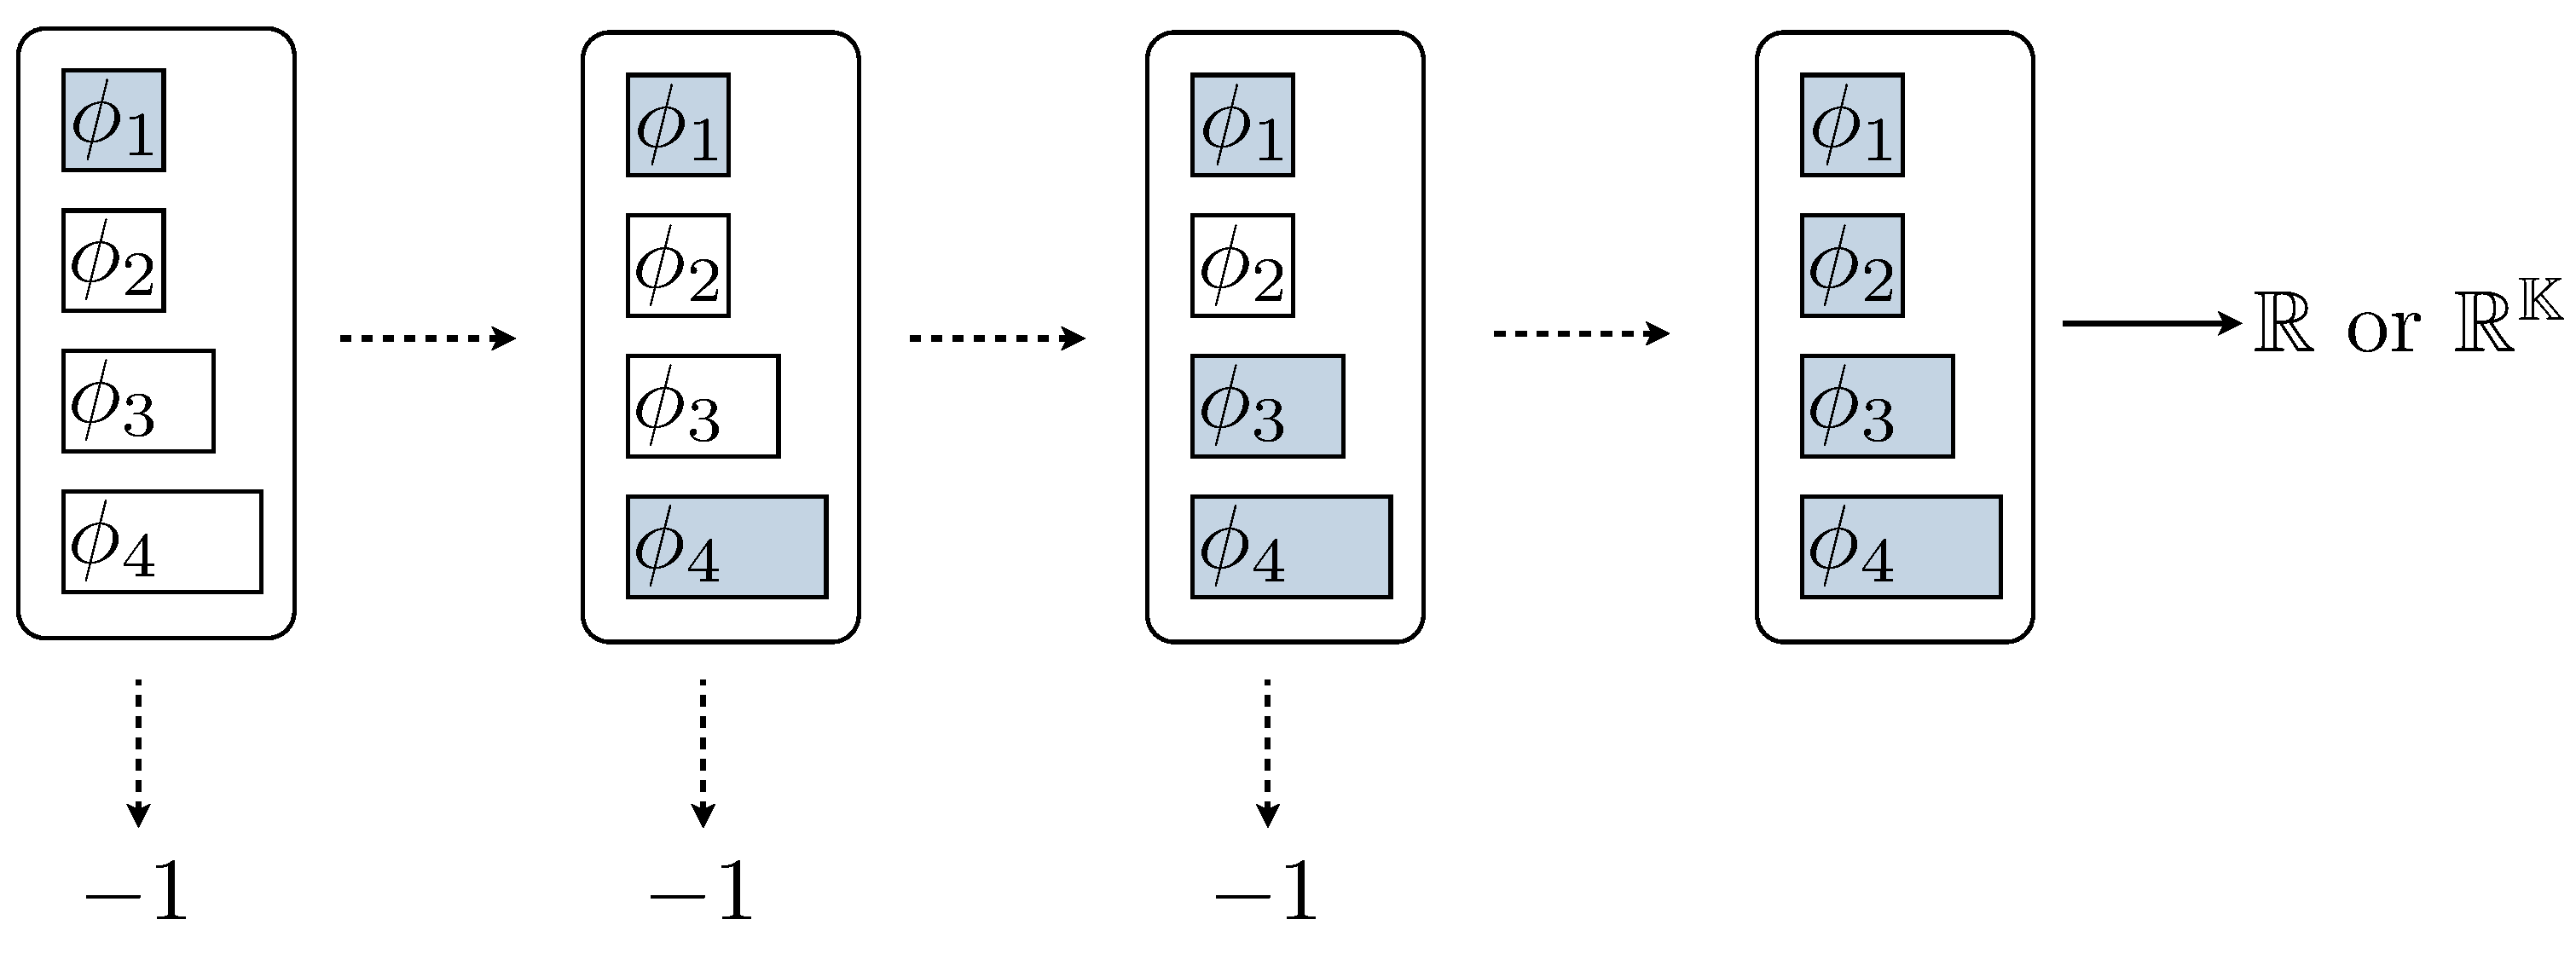
\includegraphics[width=\linewidth]{../../figures/models/cascade}
    \caption{
\textbf{Cascade}
In addition to the feature computation actions, the classifier is augmented with a rejection action.
The cascade is Anytime in a limited way, as only the rejection answer can be given before all features are evaluated.
Furthermore, the fixed order of the cascade is not robust to the fact that different images benefit from different features.
}
\end{subfigure}\hfill%
\begin{subfigure}[t]{0.48\linewidth}
    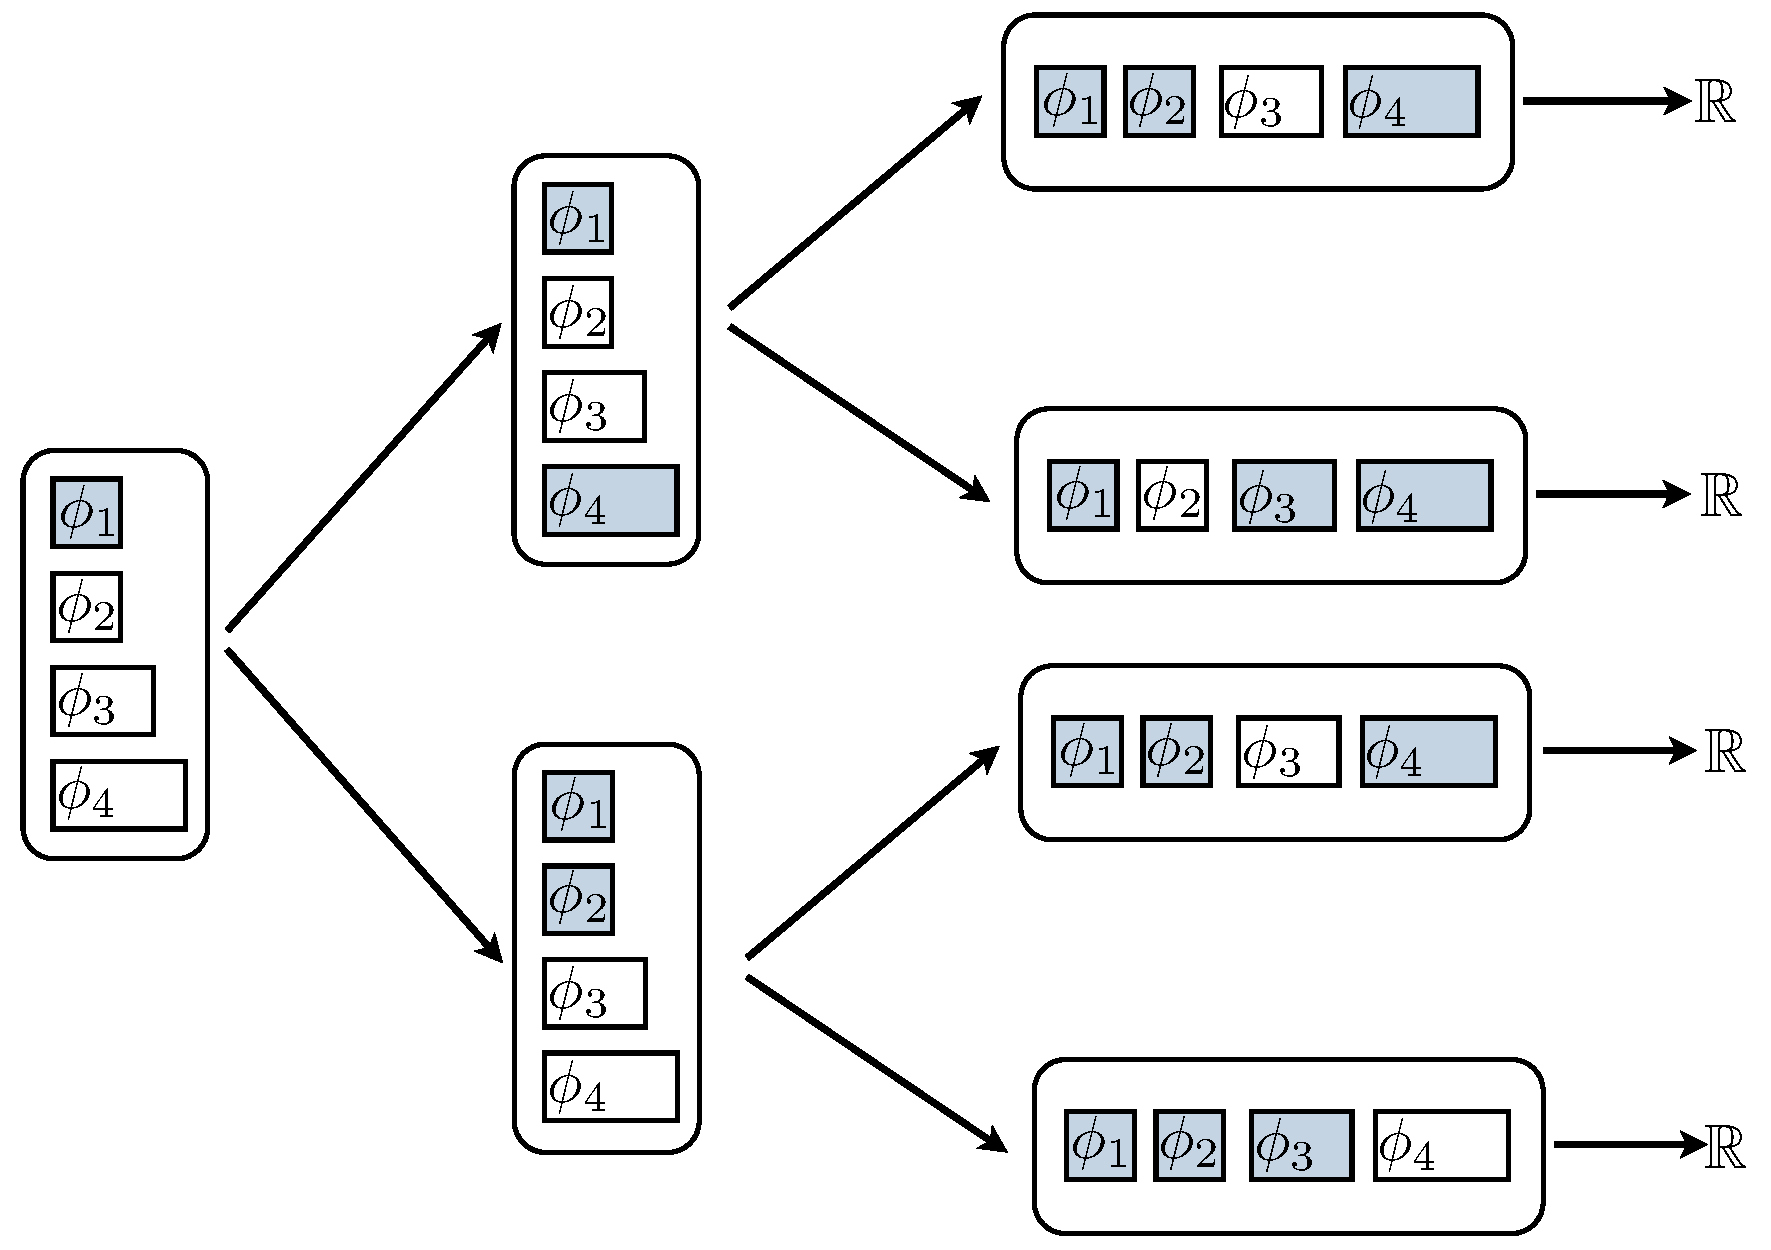
\includegraphics[width=\linewidth]{../../figures/models/tree}
    \caption{
Methods such as \cite{Xu-ICML-2012} find a tree-structured policy for computing features.
Classification answers are given only at the leaf nodes.
    }
\end{subfigure}\\
\begin{subfigure}[t]{0.48\linewidth}
    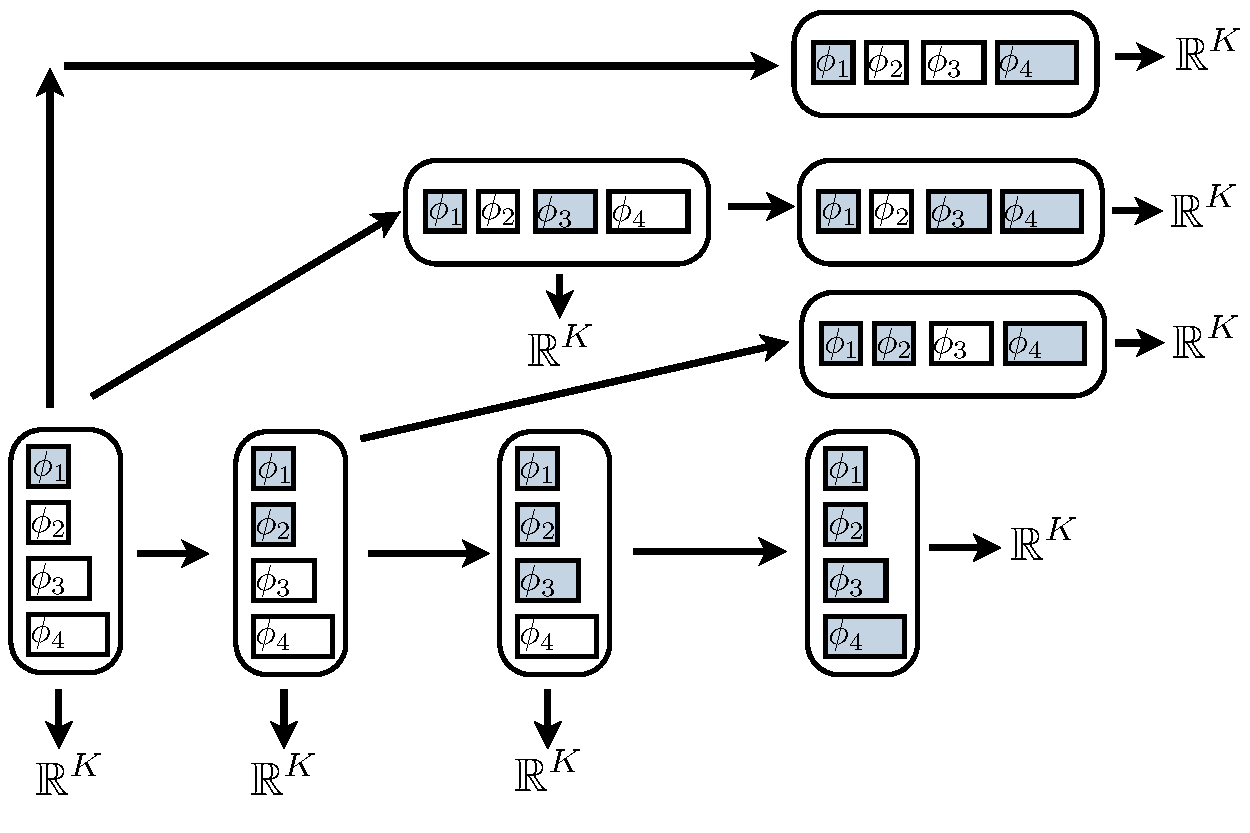
\includegraphics[width=\linewidth]{../../figures/models/benbouzid}
    \caption{
The method of \cite{Benbouzid-ICML-2012} augments the traditional cascade with an additional Skip action, which allows learning a more robust policy.
}
\end{subfigure}\hfill%
\begin{subfigure}[t]{0.48\linewidth}
    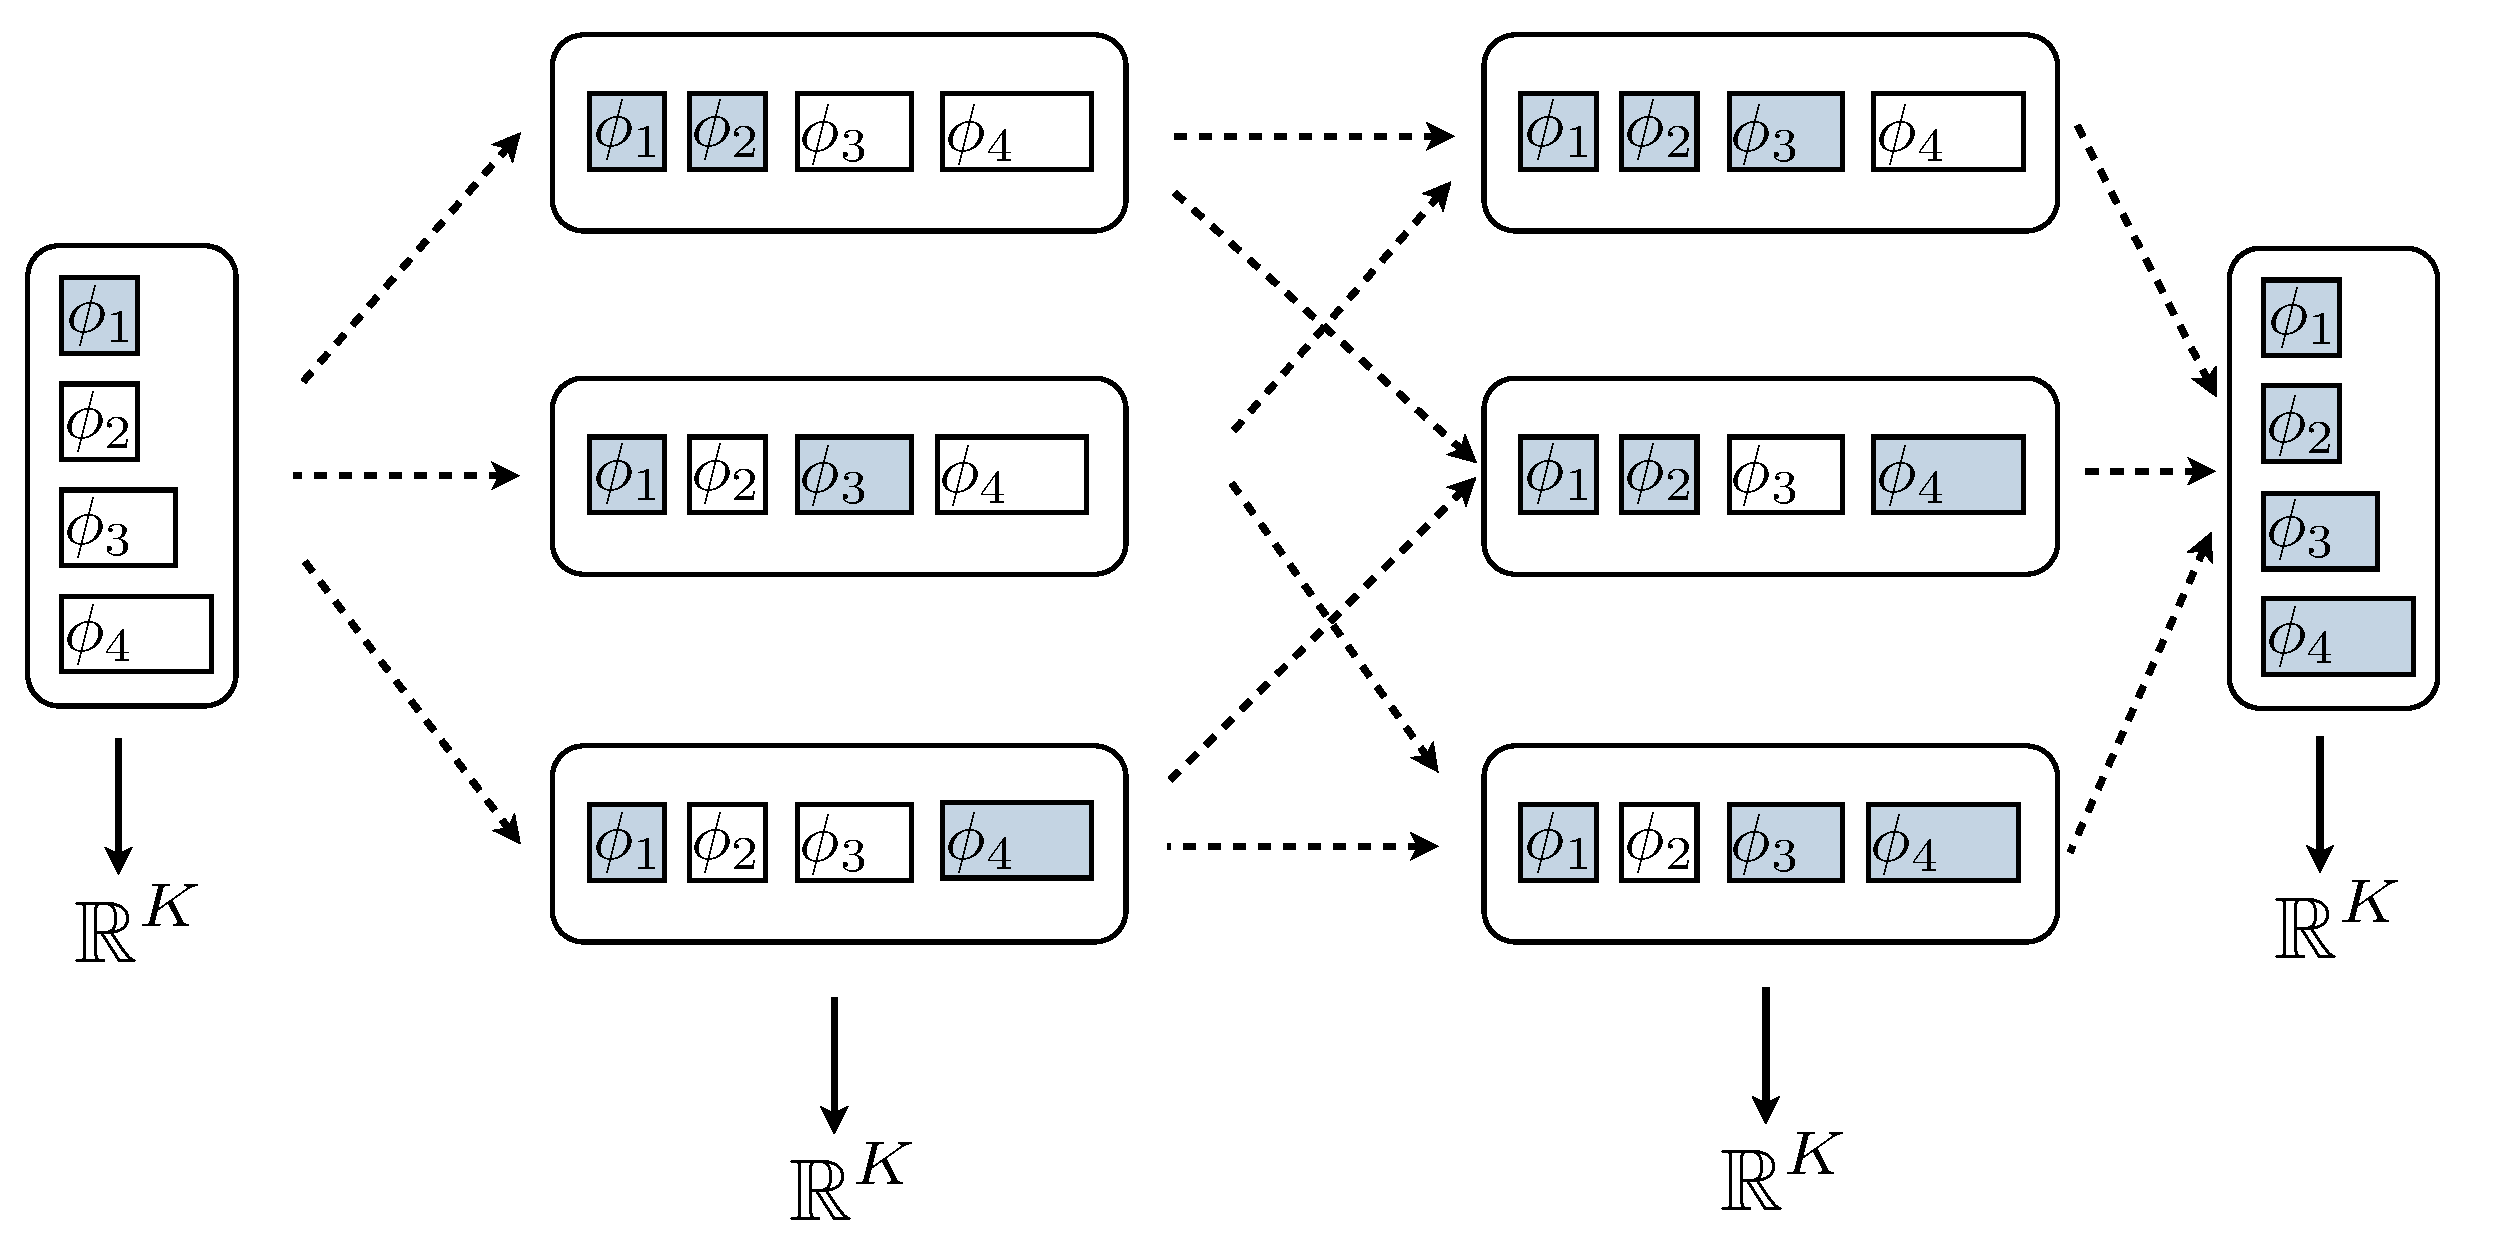
\includegraphics[width=\linewidth]{../../figures/models/dag}
    \caption{
In this work and in methods such as \cite{Gao-NIPS-2011}, the policy is a DAG over selected-feature subsets, which allows actions to be taken in an entirely flexible order.
We are also able to give the classification answer from all states, making our work truly Anytime.
    }
\end{subfigure}
\caption{
Different models for classification with sequential feature selection.
}\label{fig:models}
\end{figure}


\PM{Feature selection}
The simplest way to limit the number of features used at test time is to $L_1$-regularize.
This method does not explicitly consider feature cost, nor is it able to evaluate features one by one, or to give an answer before all features are computed.
We consider more advanced methods, all of them treating feature selection as a sequential process.
\autoref{fig:models} shows a few approaches to the problem (all additionally described below).

\PM{Cascaded methods}
A well-known method to evaluate features sequentially is the cascaded boosted classifier of \cite{Viola2004} (updated by \cite{Bourdev-CVPR-2005} with a soft threshold), which is able to quit evaluating an instance before all features are computed---but feature cost was not considered.
The cost-sensitive cascade of \cite{Chen-AISTATS-2012} optimizes stage order and thresholds to jointly minimize classification error and feature computation cost.
\cite{Xu-ICML-2012} and \cite{Grubb-AISTATS-2012} separately develop a variant of gradient boosting for training cost-sensitive classifiers; the latter prove near-optimality of their greedy algorithm with submodularity results.
Their methods are tightly coupled to the stage-wise regression algorithm.
Cascades are not dynamic policies: they cannot change the order of execution based on observations obtained during execution, which is our goal.

\PM{Dynamic methods}
In contrast, \emph{Label trees} guide an instance through a tree of classifiers; their structure is determined by the confusion matrix or learned jointly with weights \parencite{Deng-NIPS-2011}.
\cite{Xu-ICML-2013} learn a cost-sensitive binary tree of weak learners using an approach similar to the cyclic optimization of \parencite{Chen-AISTATS-2012}.
\cite{Gao-NIPS-2011} propose a method for \emph{active classification}: myopically selecting the next feature based on expected information gain given the values of the already selected features.
The method is based on locally weighted regression, highly costly at test time.
\cite{Ji-PR-2007} also formulate cost-sensitive feature selection generatively, as an HMM conditioned on actions, but select actions myopically, again at signficant test time cost.

\PM{Reinforcement Learning}
\cite{DulacArnold-ML-2012} present an MDP-based solution to ``datum-wise classification'', with an action space comprised of all features and labels, recently extended to region-based processing \parencite{DulacArnold-ICLR-2014}.
\cite{HeHe-ICMLW-2012} also formulate an MDP with features and a single classification step as actions, but solve it via imitation learning of a greedy policy.
\cite{Benbouzid-ICML-2012} formulate an MDP that simply extends the traditional sequential boosted classifier with an additional \emph{skip} action, significantly limiting the space of learnable policies.
\cite{Trapeznikov-ML-2012} provides another variation on this problem.

\PM{Misc}
Less directly related---but exciting for its novelty---is the work of \parencite{Weiss-ICCV-2013}, who apply simple introspection to structured models for a significant speedup of human pose estimation.
Another exciting direction is theoretical analysis, based on adaptive submodularity \parencite{Golovin-and-Krause-2010-JAIR} of near-optimal policies with humans in the loop \parencite{Chen-2014-ICML}.

\subsubsection{Feature Combination}

\PM{Boosting and MKL}
\emph{Boosting} is a method for combining weak learners into a more powerful classifier \parencite{Hastie2009}.
A popular use of boosting is in introducing non-linearities by training depth-limited decision trees as weak learners---the boosting trick.
For SVM-based classifiers, \emph{Multiple Kernel Learning} (MKL) provides a way to train classifiers using an automatically weighted combination of kernels \parencite{Lanckriet2004}.
It has been shown that MKL is outperformed by boosting single-kernel classifiers \parencite{Gehler2009}.
Of course, if all classifiers are linear, then combining outputs of classifiers trained on different feature channel with another classifier is equivalent to training one classifier on all features at once.

\PM{Imputing values}
The imputation problem is faced in the \emph{collaborative filtering} literature, working on problems such as the Netflix Prize \parencite{Koren-2009}.
Matrix factorization methods, commonly based on the Singular Value Decomposition (SVD), are often employed.
Our problem is significantly different in that at training time, all values are fully observed --- and the final task is classification, not simple imputation.
Imputation approaches have also been explored in genomics work, where the real-world data is often missing a large portion of the observations \parencite{Hastie-1999}.
